
\begin{quote}
\noindent {\em These notes extend our ideas of linear advection to a scalar nonlinear equation.}
\end{quote}


\section{Burgers' equation}

The inviscid Burgers' equation is the simplest {\em nonlinear} hyperbolic
equation:
\begin{equation}
u_t + u u_x = 0
\end{equation}
Here $u$ is both the quantity being advected and the speed at which 
it is moving.
In conservative form, this appears as:
\begin{equation}
u_t + \left [\tfrac{1}{2} u^2 \right ]_x = 0
\end{equation}

The solution of this follows the same methodology as outlined above.
The interface states are predicted as:
\begin{eqnarray}
u^{n+1}_{i+1/2,L} 
 &=& u^n_i + \frac{\Delta x}{2} \frac{\partial u}{\partial x}
    + \frac{\Delta t}{2} \left . \frac{\partial u}{\partial t} \right |_i
    + \ldots \\
 &=& u^n_i + \frac{\Delta x}{2} \frac{\partial u}{\partial x}
    + \frac{\Delta t}{2} \left . \left (-u_i \frac{\partial u}{\partial x} 
         \right ) \right |_i 
    + \ldots \\
 &=& u^n_i + \frac{\Delta x}{2} 
   \left ( 1 - \frac{\Delta t}{\Delta x} u_i \right ) 
   \left . \frac{\partial u}{\partial x} \right |_i + \ldots
\end{eqnarray}
The only difference with the linear advection equation is that now
$u_i \Delta t/\Delta x$ varies from zone to zone, whereas with linear
advection, it is the constant $C$.  The slopes are computed using
the same limiters as with linear advection.

The Riemann problem differs from linear advection.  It remains the
case that the solution is constant along the lines $x = ut + x_0$ (the
characteristics), but now those lines are no longer parallel.  If the
characteristic lines intersect, then there it is not possible to trace
backward from time to learn where the flow originated.  This is the 
condition for a {\em shock}.

\begin{figure}[t]
\centering
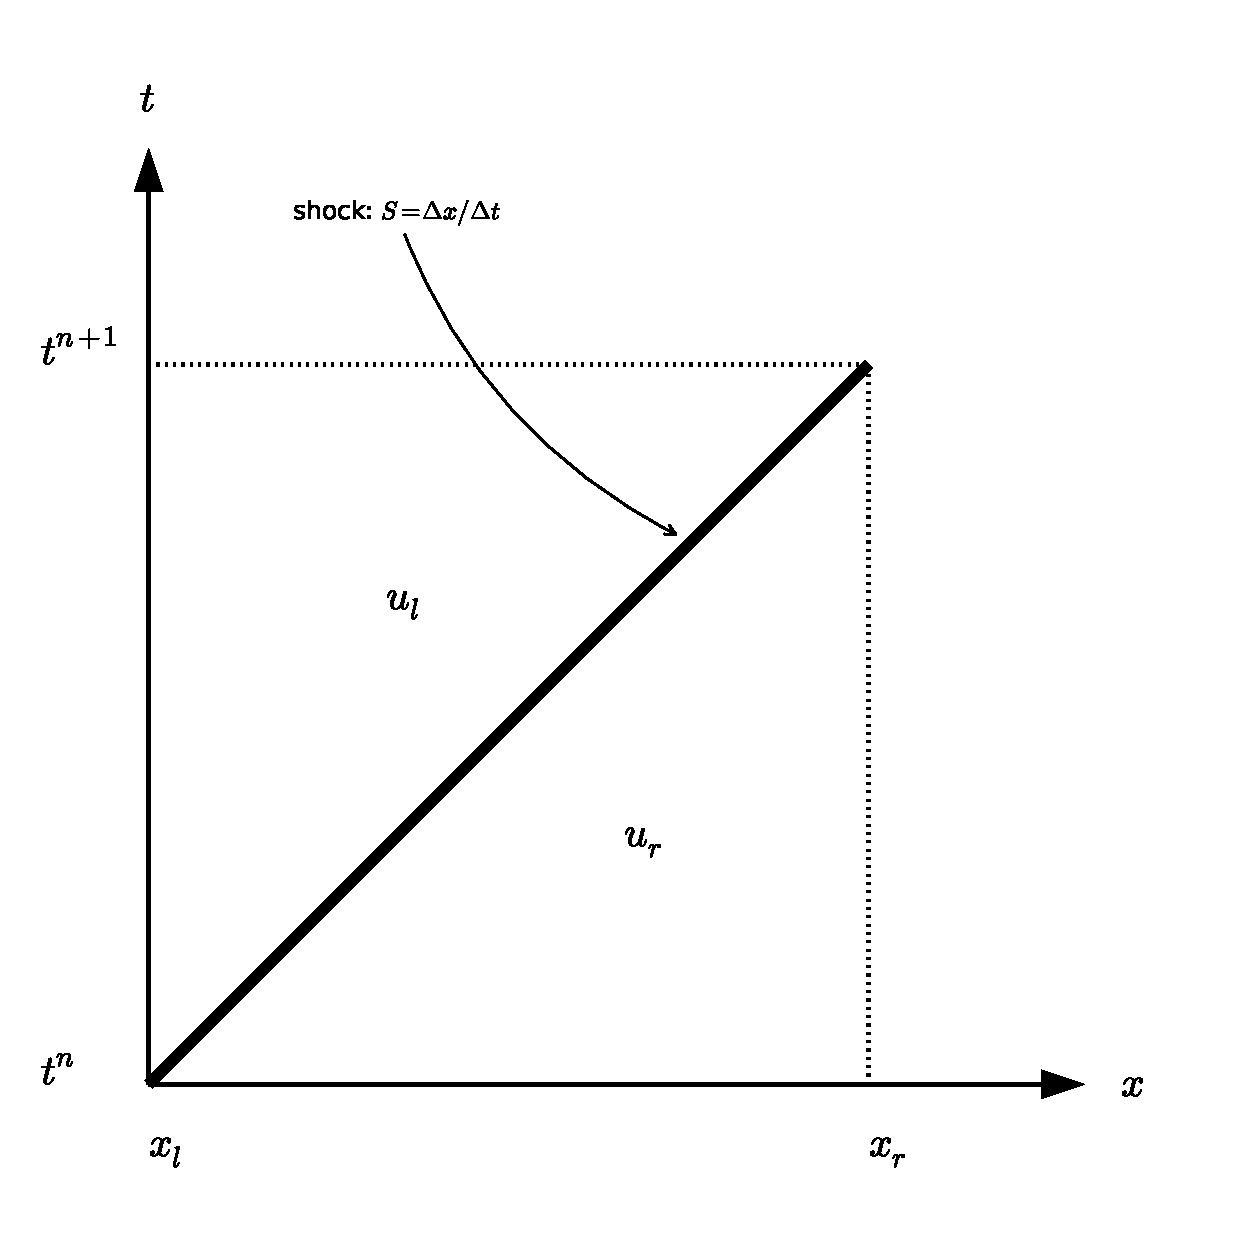
\includegraphics[width=4in]{rh}
\caption[Rankine-Hugoniot conditions]{\label{fig:rh} A rightward moving shock in the $x$-$t$
   plane separating two states: $u_l$ and $u_r$.}
\end{figure}

The shock speed is computed through the {\em Rankine-Hugoniot} jump
conditions.  For a scalar equation, these are easy to construct.
We'll follow the method of \cite{leveque:2002}.  Figure~\ref{fig:rh}
shows two states separated by a rightward moving shock in the $x$-$t$
plane.  At time $t^n$, the state in our interval ($x \in [x_l,x_r]$)
is entirely $u_r$, and at the later time, $t^{n+1}$ it is entirely
$u_l$.  The shock moves with a speed $S = \Delta x/\Delta t$ in this
figure.  To determine the speed, we integrate our conservation law over
both space and time (and normalize by $\Delta x = x_r - x_l$):
\begin{equation}
\frac{1}{\Delta x} \int_{x_l}^{x_r} dx \int_{t^n}^{t^{n+1}} dt u_t = 
  - \frac{1}{\Delta x} \int_{x_l}^{x_r} dx \int_{t^n}^{t^{n+1}} dt \left [ f(u) \right ]_x
\end{equation}
Doing the $t$ integral on the left and $x$ integral on the right, we have
\begin{equation}
\frac{1}{\Delta x} \int_{x_l}^{x_r}\left \{ u(t^{n+1}) - u(t^n) \right \} dx = 
  - \frac{1}{\Delta x} \int_{t^n}^{t^{n+1}} \left \{ f(u) |_{x=x_r} - f(u) |_{x=x_l} \right \} dt
\end{equation}
Recognizing that at $t=t^n$, $u = u_r$ and at $t=t^{n+1}$, $u = u_l$,
$\{ u(t^{n+1}) - u(t^n) \}$ in the left side becomes $\{ u_l -u_r \}$.
For the right side, we see that all along $x=x_l$ the flux is $f =
f(u_l)$ for $t\in [t^n, t^{n+1}]$.  Likewise, all along $x=x_r$, the
flux is $f = f(u_r)$ in the same time interval (see the figure).
Therefore, our expression becomes:
\begin{equation}
(u_l - u_r) = -\frac{\Delta t}{\Delta x} (f(u_r) - f(u_l)
\end{equation}
and using $S = \Delta x/\Delta t$, we see
\begin{equation}
S = \frac{f(u_r) - f(u_l)}{u_r - u_l}
\end{equation}

For Burgers' equation, substituting in $f(u) = u^2/2$, we get
\begin{equation}
S = \frac{1}{2}(u_l + u_r)
\end{equation}

With the shock speed known, the Riemann problem is straightforward.  If there
is a shock (compression, so $u_l > u_r$) then we compute the shock speed and
check whether the shock is moving to the left or right, and then use the appropriate
state.  If there is no shock, then we can simply use upwinding, as there is no
ambiguity as to how to trace backwards in time to the correct state.
Putting this together, we have:
\begin{eqnarray}
\mathrm{if~} \underset{\text{(shock)}}{u_l > u_r}:&& u_s = \left \{ \begin{array}{cl}
                u_l & \mathrm{if~} S > 0 \\ 
                u_r & \mathrm{if~} S < 0 \\
                0   & \mathrm{if~} S = 0 \end{array} \right .   \\[1em]
%
\mathrm{otherwise:}&& u_s = \left \{ \begin{array}{clc}
                u_l & \mathrm{if~} u_l \ge 0 \\  
                u_r & \mathrm{if~} u_r \le 0 \\  
                0   & \mathrm{otherwise} \end{array} \right .   
\end{eqnarray}
               
Once the interface states are constructed, the flux is calculated as:
\begin{equation}
F^{n+1/2}_{i+1/2} = \frac{1}{2} \left (u_{i+1/2}^{n+1/2} \right )^2
\end{equation}
and the conservative update is
\begin{equation}
u_i^{n+1} = u_i^n + \frac{\Delta t}{\Delta x} 
   \left ( F_{i-1/2}^{n+1/2} - F_{i+1/2}^{n+1/2} \right )
\end{equation}

The timestep constraint now must consider the most restrictive Courant 
condition over all the zones:
\begin{equation}
\Delta t = \min_i \left \{ \Delta x / u_i \right \}
\end{equation}


\begin{figure}[t]
\centering
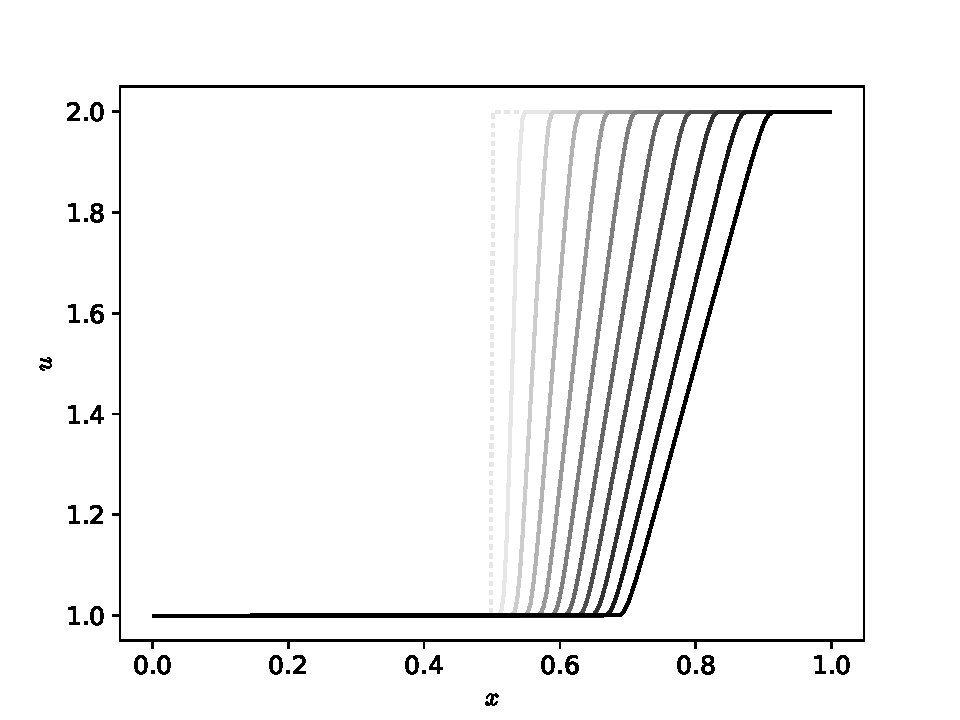
\includegraphics[width=0.475\linewidth]{fv-burger-rarefaction}
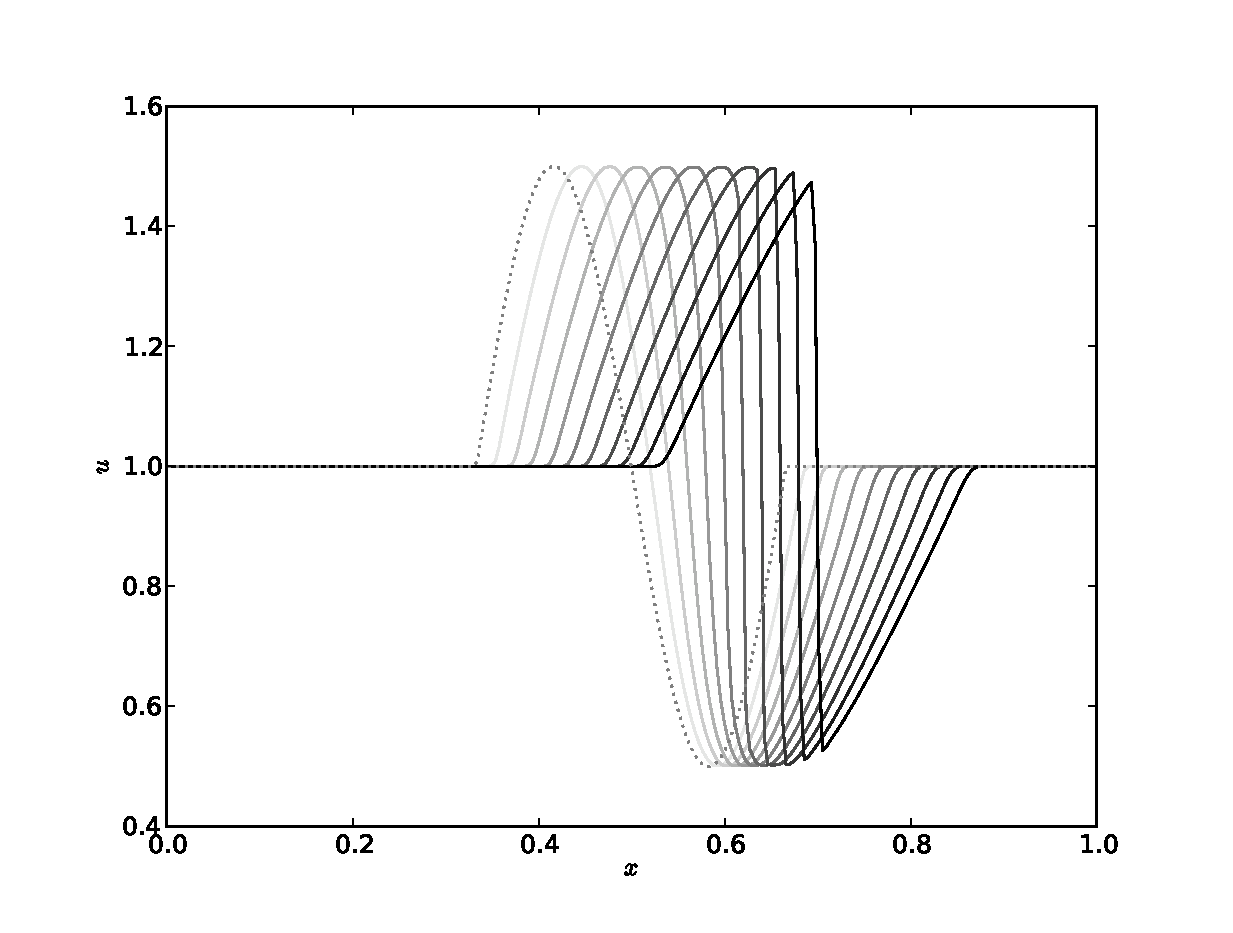
\includegraphics[width=0.475\linewidth]{fv-burger-sine}
\caption[Solutions to the inviscid Burgers'
  equation.]{\label{fig:burgers} Solution to the inviscid Burgers'
  equation with 256 zones and a Courant number, $C = 0.8$.  On the
  left, is a rarefaction---the left half of the domain was initialized
  with $u = 1$ and the right half with $u = 2$, creating a divergent
  flow.  On the right is a sine-wave steepening into a shock.  The
  curves are shown 0.02~s apart. \\
  \hydroexdoit{\href{https://github.com/zingale/hydro_examples/blob/master/burgers/burgers.py}{burgers.py}}}
\end{figure}

Figure~\ref{fig:burgers} shows the solution for two cases: a rarefaction
and a sine-wave steepening into a shock, using a piecewise linear
reconstruction and the MC limiter.

\begin{exercise}[Simple Burgers' solver]
{Extend your 1-d finite-volume solver for advection (from Exercise~\ref{adv:ex:fv}) to solver Burgers' equation.  You will need to change the Riemann solver
and use the local velocity in the construction of the interface states.  Run
the examples shown in Figure~\ref{fig:burgers}}.
\end{exercise}

\section{Going further}

\begin{itemize}
\item The equation we've been dealing with here is the {\em inviscid} Burgers' equation. 
The full Burgers' equation includes viscosity (a velocity diffusion):
\begin{equation}
u_t + u u_x = \epsilon u_{xx}
\end{equation}
To solve this, we need to first learn about techniques for diffusion, and then how to
solve equations with multiple PDE types.  This will be described later.

\end{itemize}
